%!TEX program = xelatex
% 完整编译: xelatex -> biber/bibtex -> xelatex -> xelatex
\documentclass[lang=cn,11pt,a4paper]{elegantpaper}

\title{最优化方法笔记}
\author{22120307 陈景龙}
\institute{北京交通大学}

% \version{0.10}
\date{\zhtoday}

\usepackage{algorithm}
\usepackage{algorithmic}
\usepackage{siunitx}

% 本文档命令
\usepackage{array}
\newcommand{\ccr}[1]{\makecell{{\color{#1}\rule{1cm}{1cm}}}}
\addbibresource[location=local]{./reference.bib} % 参考文献,不要删除

% 定义数学命令
\newcommand{\subject}{s.t.}
\newcommand{\E}{\mathbb{E}}
\newcommand{\I}{\mathbb{I}}
% \newcommand{\subject}{\operatorname{subject\ to}}
\newcommand{\st}{\operatorname{s.t.}}


\begin{document}

% \maketitle
% \begin{abstract}
% \end{abstract}

\newpage
\definecolor{winered}{rgb}{0,0,0} 
\tableofcontents
\newpage

\section*{重点内容}
总成绩=平时成绩(30\%)+ 小论文(20\%)+期末考试成绩(50\%)

\begin{center}
    \begin{tabular}{|l|c|}
        \hline
        \begin{tabular}{l}
            最优化问题简介、发展史、分类 \\
            无约束优化理论 \\
            无约束优化的最优性条件
        \end{tabular} & \\ \hline
        \begin{tabular}{l}
            算法概述和基础 \\
            使用导数的最优化方法, 最速下降法,牛顿法 \\
        \end{tabular} & 重点 \\ \hline
        \begin{tabular}{l}
            牛顿法, 拟牛顿法
        \end{tabular} & 重点 \\ \hline
        \begin{tabular}{l}
            共轭梯度法
        \end{tabular} & 重点 \\ \hline
        \begin{tabular}{l}
            最小二乘法
        \end{tabular} &  \\ \hline
        \begin{tabular}{l}
            约束优化理论\\
            约束优化的最优性条件, Lagrange乘子
        \end{tabular} & 重点 \\ \hline
        \begin{tabular}{l}
            约束优化的最优性条件: 二阶条件,凸规划
        \end{tabular} & 重点 \\ \hline
        \begin{tabular}{l}
            凸规划的性质、对偶理论、鞍点定理
        \end{tabular} & 重点 \\ \hline
        \begin{tabular}{l}
            线性规划的基本性质,极点和基解
        \end{tabular} & \\ \hline
        \begin{tabular}{l}
            线性规划的单纯形方法
        \end{tabular} & \\ \hline
        \begin{tabular}{l}
            约束优化问题的罚函数法
        \end{tabular} & 重点 \\ \hline
        \begin{tabular}{l}
            增广Lagrangian方法/乘子罚函数方法
        \end{tabular} & \\ \hline
    \end{tabular}
\end{center}
\section{Introduction}
\begin{note}
    给定二次型 $f(X) = X^T AX$,若对 $\forall X \neq 0$,都有 $f(X) = X^T AX > 0$ 成立,则称 $f(X)$ 为正定二次型,$A$ 为正定矩阵.

    对于 $n$ 阶实对称矩阵 $A$,下列命题等价:
    \begin{itemize}
        \item $A^T AX$ 是正定二次型(或 $A$ 是正定矩阵)
        \item $A$ 的 $n$ 个顺序主子式都大于 0
        \item $A$ 的 $n$ 个特征值都大于 0
        \item 存在可逆矩阵 $P$,使得 $A = P^T P$
    \end{itemize}
\end{note}

\begin{note}
    给定二次型 $f(X) = X^T AX$,若对 $\forall X \neq 0$,都有 $f(X) = X^T AX \ge 0$ 成立,则称 $f(X)$ 为半正定二次型,$A$ 为半正定矩阵.

    对于 $n$ 阶实对称矩阵 $A$,下列命题等价:
    \begin{itemize}
        \item $A^T AX$ 是半正定二次型(或 $A$ 是半正定矩阵)
        \item $A$ 的所有主子式都大于等于 0,而且至少有一个等于 0
        \item $A$ 的 $n$ 个特征值都大于等于 0,而且至少有一个等于 0
    \end{itemize}
\end{note}

\begin{note}
    设 $S \subseteq E^n$,若对 $\forall x, y \in S, \forall \lambda \in [0, 1]$,都有 $\lambda x + (1 - \lambda)y \in S$,则称 $S$ 为凸集.
    \begin{itemize}
        \item $x_1, \dots, x_k \in S, \lambda_1 + \cdots + \lambda_k = 1$,称 $\sum_{i = 1}^k \lambda_ix_i$ 为 $x_1, \dots, x_k$ 的凸组合
        \item $S$ 是非空凸集,$x\in S$,若由 $x = \lambda x_1 + (1 - \lambda)x_2$,其中 $\lambda \in (0, 1), x_1, x_2 \in S$,必推出 $x = x_1 = x_2$,则称 $x$ 是 $S$ 的极点.
        \item $S$ 是 $E^n$ 中的闭凸集,$d \in E^n, d \neq 0$,如果对 $\forall x \in S$,有 $\left\{x + \lambda d | \lambda > 0\right\} \subset S$,则称向量 $d$ 为 $S$ 的方向.若 $S$ 的方向 $d$ 不能表示为集合的两个不同方向的\textbf{正线性组合},则称 $d$ 为 $S$ 的极方向.
    \end{itemize}
\end{note}

\begin{note}
    设 $S = \left\{x \mid Ax = b, x \ge 0\right\}$ 为非空多面集,则有
    \begin{itemize}
        \item 极点集非空,且存在有限个极点
        \item 极方向集合为空集的充要条件是 $S$ 有界;若 $S$ 无界,则存在有限个极方向
        \item (多面集表示定理)$x \in S$ 的充要条件是 \begin{gather*}
            x = \sum_{j = 1}^k \lambda_j x^{(j)} + \sum_{j = 1}^l \mu_j d^{(j)}\\
            \lambda_j \ge 0, \forall j = 1, \dots, k\\
            \sum_{j = 1}^k \lambda_j = 1\\
            \mu_j \ge 0, \forall j = 1, \dots, l
        \end{gather*}
    \end{itemize}
\end{note}

\begin{note}
    凸集分离定理:
    \begin{itemize}
        \item 设 $S$ 为 $E^n$ 的闭凸集,$y\notin S$,则存在唯一的 $\overline{x} \in S$,使得\[ \|y - \overline{x}\| = \sideset{}{}{\operatorname{inf}}_{x \in S}\|y - x\| > 0 \]
        $\overline{x}$ 是这一最小距离点 $\Leftrightarrow (y - \overline{x})^T(\overline{x} - x) \ge 0, \forall x \in S$.

        \item 设 $S$ 是 $E^n$ 的非空闭凸集,$y\notin S$,则存在非零向量 $p$ 以及数 $\varepsilon > 0$,使得对 $\forall x \in S$,有 $p^T y \ge \varepsilon + p^T x$
        
        \item 设 $S$ 是 $E^n$ 的非空凸集,$y\in \partial S$,则存在非零向量 $p$,使得对 $\forall x \in clS$($S$ 的闭包,由 $S$ 的内点和边界点组成),有 $p^Ty \ge p^Tx$.
        
        \item 设 $S_1$ 和 $S_2$ 是 $E^n$ 的两个非空凸集,$S_1 \cap S_2 = \varnothing$,则存在非零向量,使得\[p^Ty \ge p^T x \quad \text{其中}\forall y \in S_1, \forall x \in S_2\]
    \end{itemize}
\end{note}

\begin{note}
    两个系统恰有一个有解:
    \begin{itemize}
        \item Farkas 引理:设 $A$ 为 $m\times n$ 矩阵,$c$ 为 $n$ 维列向量,则 $Ax \le 0, c^Tx > 0$ 有解的充分条件是 $A^Ty = c, y\ge 0$ 无解.
        \item Gordan定理:给定矩阵 $\boldsymbol{A} \in \mathbb{R}^{m\times n}$,下列两个系统只有一个有解
        \begin{gather*}
            \boldsymbol{A}x < 0\\
            \boldsymbol{y} \ge 0, \boldsymbol{y} \neq 0, \boldsymbol{A}^T\boldsymbol{y} = 0
        \end{gather*}
    \end{itemize}
\end{note}

\begin{note}
    设 $S$ 是 $E^n$ 中的非空凸集,$f(x)$ 是定义在 $S$ 上的实函数,如果对于每一对 $x_1, x_2 \in S$ 及每一个 $\lambda, 0\le \lambda \le 1$ 都有 \[f(\lambda x_1 + (1 - \lambda)x_2) \le \lambda f(x_1) + (1 - \lambda)f(x_2)\]
    则称函数 $f(x)$ 为 $S$ 上的凸函数.

    凸函数的根本重要性:设 $S$ 是 $E^n$ 中的非空凸集,$f$ 是定义在 $S$ 上的凸函数,则 $f$ 在 $S$ 上的局部极小点事整体极小点,且极小点的集合是凸集.
\end{note}

\begin{note}
    $f(x)$ 是凸集 $S$ 上的凸函数,对每一个实数 $c$,则集合 $S_c = \left\{x | x \in S, f(x) \le c\right\}$ 是凸集.
\end{note}

\begin{note}
    凸函数的判别:
    \begin{itemize}
        \item (一阶充要条件)设 $S$ 是 $E^n$ 中的非空开凸集,$f(x)$ 是定义在 $S$ 上的\textbf{可微}函数,则 $f(x)$ 为凸函数的充要条件是对任意两点 $x_1, x_2 \in S$,有 \[f(x_2) \ge f(x_1) + \nabla f(x_1)^T(x_2 - x_1)\]
        $f(x)$ 为严格凸函数的充要条件是对任意互不相同两点 $x_1, x_2 \in S$,有 \[f(x_2) > f(x_1) + \nabla f(x_1)^T(x_2 - x_1)\]

        几何意义:$f(x)$ 是凸函数当且仅当任意点处的切线增量不超过函数的增量.
        \item (二阶充要条件)设 $S$ 是 $E^n$ 中的非空开凸集,$f(x)$ 是定义在 $S$ 上的\textbf{二次可微}函数,则 $f(x)$ 为凸函数的充要条件是对任意 $x \in S$,$f(x)$ 在 $x$ 处的Hessian矩阵 $\nabla ^2f(x)$ 是半正定的.
        
        $f(x)$ 为严格凸函数的充要条件是对任意 $x \in S$,$f(x)$ 在 $x$ 处的Hessian矩阵 $\nabla ^2f(x)$ 是正定的.
    \end{itemize}
\end{note}

\begin{note}
    设 $f(x)$ 是定义在凸集 $S$ 上的可微凸函数,若 $\exists x^* \in S$,使对 $\forall x \in S$,都有 \[\nabla f(x^*)^T(x - x^*) \ge 0\]
    则 $x^*$ 是 $f(x)$ 在凸集 $S$ 上的全局极小点.
\end{note}

\begin{note}
    凸规划:求凸函数在凸集上的极小点.
    \begin{align*}
        \min \quad &f(x)\\ 
        s.t. \quad &g_{i}(x) \le 0, i=1, \cdots, m \\  
        &h_{j}(x)=0, j=1, \cdots, l 
    \end{align*}
    若 $f(x)$ 是凸函数,$g_i(x)$ 是凸函数,$h_j(x)$ 是线性函数,则原问题为凸规划.
    \begin{itemize} 
        \item 凸规划的局部极小点就是整体极小点
        \item 且极小点的集合为凸集
    \end{itemize}
\end{note}
\newpage
\section{LP 基本性质}
LP:线性规划.

\begin{definition}
    LP 标准型:
    \begin{enumerate}
        \item 极小化型
        \item 约束方程为等式
        \item 所有的决策变量为非负值
        \item 约束方程的右端项系数为非负值
    \end{enumerate}
    \begin{align*}
        \min \quad &z = c^tx\\
        \subject \quad &Ax = b\\
        &x \ge 0\\
        &c, x \in \R^n, b \in \R^m_+, A \in \R^{m \times n}
    \end{align*}
\end{definition}

\begin{note}
    LP 基本定理:
    \begin{itemize}
        \item 可行域的极点对应 LP 问题的基本可行解
        \item LP 的最优解一定可以在基本可行解中找到
        \item 设 $S$ 是 LP 的可行域,$\bar{x} \in S$,则 $\bar{x}$ 是 $S$ 的极点 $\Longleftrightarrow \bar{x}$ 是 LP 的基本可行解
        \item 如果LP有可行解,则一定存在基本可行解
        \item 如果LP有最优解,则存在一个基本可行解是最优解
        \item 若LP问题有最优解,则要么最优解唯一,要么有无
        穷多最优解
    \end{itemize}
\end{note}
\newpage
\section{单纯形法}
\subsection{单纯形法}
\begin{note}
    最优解一定在极点达到,而极点对应于基本可行解,求解线性规划问题归结为找最优基本可行解。\textbf{可以从一个基本可行解出发,求一个使目标函数值有所改善的基本可行解}:通过最优性条件判断是否达到最优解,并不断改进基本可行解,力图达到最优基本可行解。
\end{note}

\begin{note}
    对于线性规划问题
    \[
        (LP)\begin{cases}
            \min & f(x)=cx \\
            \subject & Ax=b \\
            & x \ge 0
        \end{cases}
    \]
    其中 $A$ 是 $m \times n$ 矩阵,秩为 $m$,$c$ 是 $n$ 维列向量,$b\ge 0$ 是 $m$ 维列向量.
    \begin{itemize}
        \item 初始基本可行解
            $A = (P_1, \dots, P_m, P_{m + 1}, \dots, P_n) = \begin{pmatrix}
                B & N
            \end{pmatrix}$

            基本解 $x^{(0)} = \begin{pmatrix}
                B^{-1}b \\
                0
            \end{pmatrix}$,若 $B^{-1}b \ge 0$,则 $x^{(0)}$ 是基本可行解.

            目标函数 $f_0 = cx^{(0)} = \begin{pmatrix}
                C_B & C_N
            \end{pmatrix} \begin{pmatrix}
                B^{-1}b \\
                0
            \end{pmatrix} = C_BB^{-1}b$
        \item 从初始基本可行解出发,求一个改进的基本可行解.
        \item 进基和终止条件
            \[
                x=\begin{pmatrix}
                    x_{B} \\
                    x_{N}
                \end{pmatrix}, Ax=b \Rightarrow\begin{pmatrix}
                    B & N
                \end{pmatrix}\begin{pmatrix}
                    x_{B} \\
                    x_{N}
                \end{pmatrix}=B x_{B}+N x_{N}=b \Rightarrow x_{B}=B^{-1}b-B^{-1} Nx_{N}
            \]
            目标函数值:
            \begin{align*}
                f = cx &= \begin{pmatrix}
                    c_B & c_N
                \end{pmatrix}\begin{pmatrix}
                    x_B \\
                    x_N
                \end{pmatrix} = c_Bx_B + c_Nx_N \\
                &= c_B(B^{-1}b - B^{-1}Nx_N) + c_Nx_N \\
                &= c_BB^{-1}b - (c_BB^{-1}N - c_N)x_N \\
                &= f_0 - \sum_{j\in R}(c_BB^{-1}P_j - c_j)x_j \quad R :\text{非基变量下标集} \\
                &=f_0 - \sum_{j\in R}(z_j - c_j)x_j
            \end{align*}
            \begin{enumerate}
                \item $z_j - c_j$ 称为检验数或判别数,基变量的检验数为0。
                \item 如果 $\forall j\in R$,有 $z_j - c_j \le 0$,则 $x^{(0)}$ 为最优解;
                \item 否则 $z_k - c_k = \underset{j \in R}{\max}\left\{z_j - c_j\right\}$,$P_k$ 为进基向量,$x_k$ 为进基变量,$x_k = 0 \to x_k > 0$.
            \end{enumerate}
        \item 出基下标和进基变量的值
        
            $Ax = b$ 解的变化,原 $x_B = B^{-1}b - B^{-1}Nx_N$,$x_k$ 由 0 变为正以后,$x_B = B^{-1}b - B^{-1}P_kx_k$,$x_B = \bar{b}-y_{k} x_{k}$,其中 $\bar{b} = B^{-1}b,y_k = B^{-1}P_k$.
            \begin{enumerate}
                \item 若 $y_{ik}\le 0$,则 $\forall x_k \Longrightarrow x_{B_i} > 0,x_k$ 可以取无限大,故 $f\to -\infty$,原问题无界.
                \item 要满足 $x_B = \bar{b}-y_{k} x_{k} \ge 0$,则取 $x_k = \min(\frac{\bar{b}}{y_{ik}},y_{ik}>0) = \frac{\bar{b}}{y_{rk}} > 0$,$r$ 为出基下标.
            \end{enumerate}
    \end{itemize}
\end{note}

\begin{note}
    单纯形法计算步骤
    \begin{enumerate}
        \item 初始基为 $B$,初始基本可行解为 $x^{(0)} = (B^{-1}b, 0)^t$,$\bar{b} = B^{-1}b$;
        \item 判断是否所有的 $c_BB^{-1}P_j - c_j \le 0$,即检验数是否全部非正,如果是,那么 $x^{(0)}$ 就是最优解,结束流程;
        \item 否则取 $z_k - c_k = \max\{z_j - c_j\} > 0$,判断是否 $y_k = B^{-1}P_k \le 0$,如果是,则解无界;
        \item 否则取 $\frac{\bar{b_r}}{y_{rk}} = \min\{\frac{\bar{b}_i}{y_{ik}} \mid y_{ik} > 0\}$,以 $p_k$ 代替 $P_{b_r}$ 换基,即 $x_{b_r}$ 为离基变量,$x_k$ 为进基变量,跳转步骤2。
    \end{enumerate}
\end{note}

\begin{note}
    单纯形表
    \begin{itemize}
        \item 做初等行变换
        \item 若 $z_j - c_j > 0$,对应的系数列向量 $\le 0$,则该 LP 存在无界解;
        \item 若某个非基变量的检验数为 0,则该 LP 存在多个最优解.
    \end{itemize}
    \begin{figure}[htbp]
        \centering
        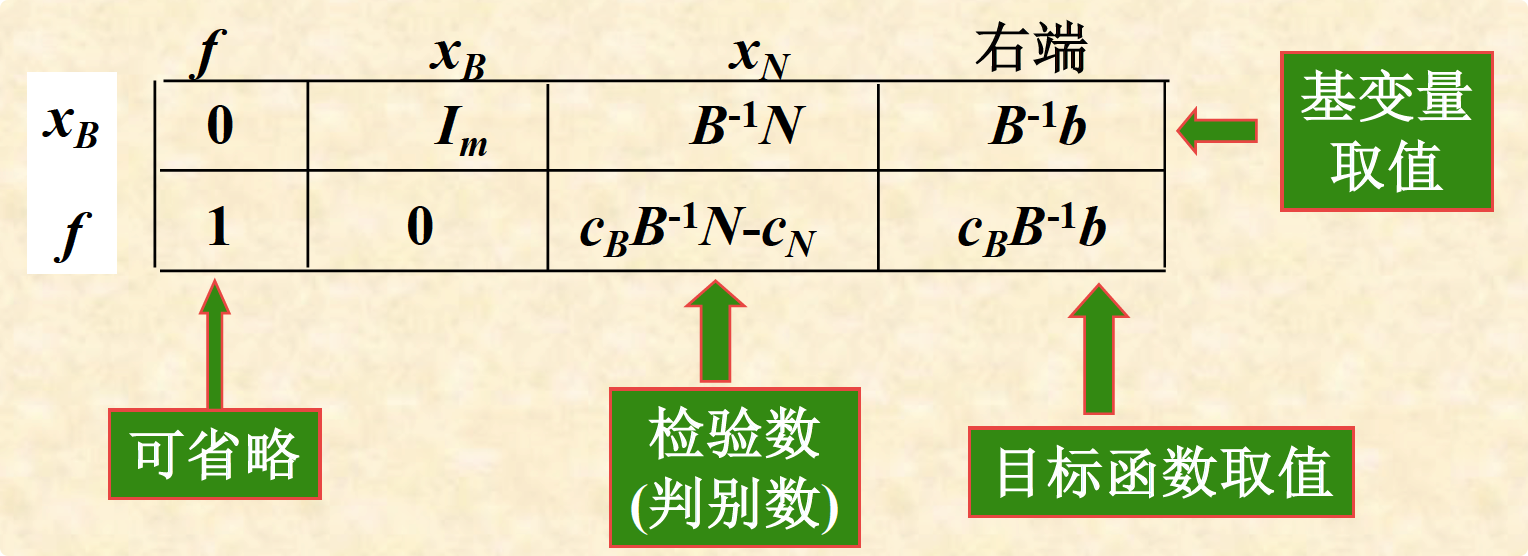
\includegraphics[width=0.8\textwidth]{./figures/img1.png}
        \caption{单纯形表 \label{fig1}}
    \end{figure}
\end{note}

\begin{example}
    用单纯形法求最优解
    \[
        \begin{cases}
            \min \quad &-x_2 + 2x_3\\
            \subject \quad &x_1 - 2x_2 + x_3 = 2\\
            &x_2 - 3x_3 \le 1\\
            &x_2 - x_3 \le 2\\
            &x_1, x_2, x_3 \ge 0
        \end{cases}  
    \]

    \answer 引入松弛变量化为标准形
    \[
        \begin{cases}
            \min \quad &-x_2 + 2x_3\\
            \subject \quad &x_1 - 2x_2 + x_3 = 2\\
            &x_2 - 3x_3 + x_4 = 1\\
            &x_2 - x_3 + x_5 = 2\\
            &x_1, x_2, x_3, x_4, x_5 \ge 0
        \end{cases}    
    \]
    选择初始基 $B = (P_1, P_4, P_5) = I$。
    \begin{center}
        \begin{tabular}{c|ccccc|c}
            & $x_1$ & $x_2$ & $x_3$ & $x_4$ & $x_5$ & \\
            \hline
            $x_1$ & 1 & -2 & 1 & 0 & 0 & 2\\
            $x_4$ & 0 & {\color{red} 1} & -3 & 1 & 0 & 1\\
            $x_5$ & 0 & 1 & -1 & 0 & 1 & 2\\
            \hline
             & 0 & 1 & -2 & 0 & 0 & 0
        \end{tabular}

        选取检验数最大的列,最大的列中 $\frac{1}{1} < \frac{2}{1}$

        \begin{tabular}{c|ccccc|c}
            & $x_1$ & $x_2$ & $x_3$ & $x_4$ & $x_5$ & \\
            \hline
            $x_1$ & 1 & 0 & -5 & 2 & 0 & 4\\
            $x_2$ & 0 & 1 & -3 & 1 & 0 & 1\\
            $x_5$ & 0 & 0 & {\color{red} 2} & -1 & 1 & 1\\
            \hline
            & 0 & 0 & 1 & -1 & 0 & -1
        \end{tabular}
        
        选取检验数最大的列,最大的列中只有 $\frac{1}{2}$可选

        \begin{tabular}{c|ccccc|c}
            & $x_1$ & $x_2$ & $x_3$ & $x_4$ & $x_5$ & \\
            \hline
            $x_1$ & 1 & 0 & 0 & -1/2 & 5/2 & 13/2\\
            $x_2$ & 0 & 1 & 0 & -1/2 & 3/2 & 5/2\\
            $x_3$ & 0 & 0 & 1 & -1/2 & 1/2 & 1/2\\
            \hline
             & 0 & 0 & 0 & -1/2 & -1/2 & -3/2
        \end{tabular}
    \end{center}
    可得 $x^* = \left(\frac{13}{2}, \frac{5}{2}, \frac{1}{2}\right)^t$,$f_{\min} = -\frac{3}{2}$。
\end{example}

\begin{example}
    用单纯形法求最优解
    \[
        \begin{cases}
            \max \quad &2x_1 + x_2 - x_3\\
            \subject \quad &x_1 + x_2 + 2x_3 \le 6\\
            &x_1 + 4x_2 - x_3 \le 4\\
            &x_1, x_2, x_3 \ge 0
        \end{cases}    
    \]
    引入松弛变量化为标准形
    \[
        \begin{cases}
            \max \quad &2x_1 + x_2 - x_3\\
            \subject \quad &x_1 + x_2 + 2x_3 + x_4 = 6\\
            &x_1 + 4x_2 - x_3 + x_5 = 4\\
            &x_1, x_2, x_3, x_4, x_5 \ge 0
        \end{cases}    
    \]
    选择初始基 $B = (P_4, P_5) = I$。
    \begin{center}
        \begin{tabular}{c|ccccc|c}
            & $x_1$ & $x_2$ & $x_3$ & $x_4$ & $x_5$ & \\
            \hline
            $x_4$ & 1 & 1 & 2 &1 & 0 & 6\\
            $x_5$ & {\color{red} 1} & 4 & -1 & 0 & 1 & 4\\
            \hline
             & -2 & -1 & 1 & 0 & 0 & 0
        \end{tabular}

        选取检验数最小的列,其中 $\frac{4}{1} < \frac{6}{1}$

        \begin{tabular}{c|ccccc|c}
            & $x_1$ & $x_2$ & $x_3$ & $x_4$ & $x_5$ & \\
            \hline
            $x_4$ & 0 & -3 & {\color{red}3} & 1 & -1 & 2\\
            $x_1$ & 1 & 4 & -1 & 0 & 1 & 4\\
            \hline
             & 0 & 7 & -1 & 0 & 2 & 8
        \end{tabular}

        选取检验数最小的列,只有 $\frac{3}{2}$

        \begin{tabular}{c|ccccc|c}
            & $x_1$ & $x_2$ & $x_3$ & $x_4$ & $x_5$ & \\
            \hline
            $x_4$ & 0 & -1 & 1 & 1/3 & -1/3 & 2/3\\
            $x_1$ & 1 & 3 & 0 & 1/3 & 2/3 & 14/3\\
            \hline
             & 0 & 6 & 0 & 1/3 & 5/3 & 26/3
        \end{tabular}
    \end{center}
    故 $x^* = \left(\frac{14}{3}, 0, \frac{2}{3}\right)^t$,$f_{\max} = \frac{26}{3}$。
\end{example}

\subsection{两阶段法}
(感觉很useless啊)

对于如下线性规划问题
\[
    \begin{cases}
        \min \quad &c^tx\\
        \subject \quad &Ax = b\\
        &x \ge 0
    \end{cases}    
\]
两阶段法步骤:
\begin{enumerate}
    \item 用单纯形法把人工变量变为非基变量,求出原问题的一个基本可行解。

    求解下列模型
    \[
        \begin{cases}
            \min \quad &e^tx_a\\
            \subject \quad &Ax + x_a = b\\
            &e = (1, \dots, 1)^t\\
            &x, x_a \ge 0
        \end{cases}
    \]
    得到最优解为 $(\bar{x}^t, \bar{x}_a^t)^t$,最优值为 $e^t\bar{x}_a$。
    \begin{enumerate}
        \item 若 $\bar{x}^a \neq 0$,则无可行解
        \item $\bar{x}_a = 0$ 而且所有的人工变量都是非基变量,则 $\bar{x}$ 是基本可行解
        \item $\bar{x}_a = 0$ 但 $\bar{x}_a$ 的某个分量 $\bar{x}_{a_j}$ 为基变量,则设法将 $\bar{x}_{a_j}$ 从基变量中去掉。
    \end{enumerate}
    \item 从得到的基本可行解出发,用单纯形法求最优解。
\end{enumerate}

\subsection{线性规划的最优性条件}
即KKT条件。

对于如下凸优化问题
\[
    \begin{cases}
        \min \quad &f(x)\\
        \subject \quad &f_i(x) \le 0, 1 \le i \le m\\
        &h_i(x) = 0, 1 \le i \le p
    \end{cases}    
\]
有拉格朗日函数 $L(x, \lambda, \mu) = f(x) + \sum \lambda_if_i(x) + \sum \mu_ih_i(x)$.

$x$ 是最优解当且仅当
\begin{enumerate}
    \item 满足约束条件:$f_i(x) \le 0$,$h_i(x) = 0$
    \item 非负约束:$\lambda \succeq 0$
    \item 互补松弛:$\lambda_if_i(x) = 0$
    \item $\partial_xL(x, \lambda, \mu) = 0$
\end{enumerate}\newpage
\section{对偶理论}
\subsection{LP 对偶问题的形式}
\begin{note}
    \figref{fig2}中,左边是对偶问题 (D),右边是原问题 (P)。
    \begin{figure}[htbp]
        \centering
        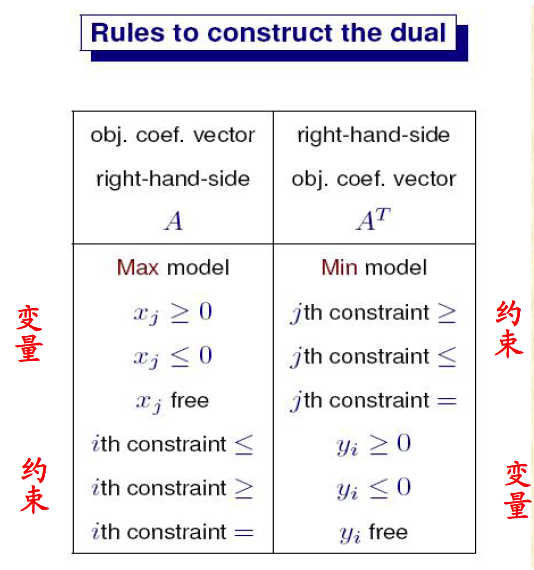
\includegraphics[width=0.4\textwidth]{./figures/img2.png}
        \caption{LP 问题的对偶问题转换规则 \label{fig2}}
    \end{figure}
    \[\begin{cases}
        \min \quad & 2x_1 + x_2 + 2x_3\\
        s.t. \quad & x_1 + x_2 + 2x_3 \ge 1\\
        &x_1 - x_2 + x_3 \le 2\\
        &-x_1 + x_2 + x_3 = 1\\
        &x_1 \ge 0, x_2 \ \text{free}, x_3 \le 0
    \end{cases} \Longrightarrow \begin{cases}
        \max \quad & w_1 + 2w_2 + w_3\\
        s.t. \quad & w_1 + w_2 - w_3 \le 2\\
        &w_1 - w_2 + w_3 = 1\\
        &2w_1 + w_2 + w_3 \ge 2\\
        &w_1 \ge 0, w_2 \le 0, w_3 \ \text{free}
    \end{cases}\]
    \begin{itemize}
        \item 原问题的变量对应对偶问题的约束,并且\textbf{符号改变}。
        \item 原问题的约束对应对偶问题的变量,符号保持,等号对应 free。
    \end{itemize}
\end{note}

\subsection{对偶问题的基本性质}
\begin{minipage}[c]{15em}
    \[
        \text{原问题 (P)}
        \begin{cases}
            \min \quad &c^tx\\
            \subject \quad &Ax \ge b\\
            &x \ge 0
        \end{cases}
    \]
\end{minipage}
\begin{minipage}[c]{15em}
    \[
        \text{对偶问题 (D)}
        \begin{cases}
            \max \quad &b^tw\\
            \subject \quad &A^tw \le c\\
            &w \ge 0
        \end{cases}
    \]
\end{minipage}

\begin{theorem}[弱对偶定理]
    弱对偶定理:若 $x^{(0)}, w^{(0)}$ 分别是原问题 (P) 和对偶问题 (D) 的可行解,则 $c^Tx^{(0)} \ge b^Tw^{(0)}$,即最小化目标的函数值大于等于最大化目标的函数值。
\end{theorem}

\begin{theorem}[弱对偶推论]
    若问题 (P) 或 (D) 有无界解,则其对偶问题 (D) 或 (P) 无可行解。
\end{theorem}

\begin{theorem}[最优性准则]
    若 $x^{(0)}$,$w^{(0)}$ 分别为 (P),(D) 的可行解且 $c^tx^{(0)} = b^tw^{(0)}$,则 $x^{(0)}$,$w^{(0)}$ 分别为 (P),(D) 问题的最优解。
\end{theorem}

\begin{theorem}[强对偶定理]
    若原问题 (P) 和对偶问题 (D) 均有可行解,则原问题 (P) 和对偶问题 (D) 均有最优解,且 (P) 和 (D) 的最优目标函数值相等。\begin{itemize}
        \item 推论:若问题 (P) 或 (D) 无可行解,则其对偶问题 (D) 或 (P) 或者无可行解,或者目标函数值趋于无穷。
        \item 推论:在用单纯形法求解 LP 问题 (P) 的松弛变量的检验数的相反数为对偶问题 (D) 的最优解。
        \item 推论:在用单纯形法求解 LP 问题 (D) 的松弛变量的检验数的为原问题 (P) 的最优解。
    \end{itemize}
\end{theorem}

\begin{example}
    求下列问题对偶问题的最优解
    \[
        \begin{cases}
            \max \quad &2x_1 + 3x_2\\
            \subject \quad &x_1 + 2x_2 \le 8\\
            &4x_1 \le 16\\
            &4x_2 \le 12\\
            &x_1, x_2 \ge 0
        \end{cases}    
    \]

    \answer
    化为标准形
    \[
        \begin{cases}
            \max \quad &2x_1 + 3x_2\\
            \subject \quad &x_1 + 2x_2 + x_3 = 8\\
            &4x_1 + x_4 = 16\\
            &4x_2 + x_5 = 12\\
            &x_1, x_2, x_3, x_4, x_5 \ge 0
        \end{cases}    
    \]

    \begin{center}
        \begin{tabular}{c|ccccc|c}
            & $x_1$ & $x_2$ & $x_3$ & $x_4$ & $x_5$ & \\
            \hline
            $x_3$ & 1 & 2 & 1 & 0 & 0 & 8\\
            $x_4$ & 4 & 0 & 0 & 1 & 0 & 16\\
            $x_5$ & 0 & {\color{red} 4} & 0 & 0 & 1 & 12\\
            \hline
            & -2 & -3 & 0 & 0 & 0 & 0
        \end{tabular}

        \begin{tabular}{c|ccccc|c}
            & $x_1$ & $x_2$ & $x_3$ & $x_4$ & $x_5$ & \\
            \hline
            $x_3$ & {\color{red} 1} & 0 & 1 & 0 & -1/2 & 2\\
            $x_4$ & 4 & 0 & 0 & 1 & 0 & 16\\
            $x_2$ & 0 & 1 & 0 & 0 & 1/4 & 3\\
            \hline
            & -2 & 0 & 0 & 0 & 3/4 & 9
        \end{tabular}

        \begin{tabular}{c|ccccc|c}
            & $x_1$ & $x_2$ & $x_3$ & $x_4$ & $x_5$ & \\
            \hline
            $x_1$ & 1 & 0 & 1 & 0 & -1/2 & 2\\
            $x_4$ & 0 & 0 & -4 & 1 & {\color{red} 2} & 8\\
            $x_2$ & 0 & 1 & 0 & 0 & 1/4 & 3\\
            \hline
            & 0 & 0 & 2 & 0 & -1/4 & 13
        \end{tabular}

        \begin{tabular}{c|ccccc|c}
            & $x_1$ & $x_2$ & $x_3$ & $x_4$ & $x_5$ & \\
            \hline
            $x_1$ & 1 & 0 & 0 & 1/4 & 0 & 4\\
            $x_5$ & 0 & 0 & -2 & 1/2 & 1 & 4\\
            $x_2$ & 0 & 1 & 1/2 & -1/8 & 0 & 2\\
            \hline
            & 0 & 0 & 3/2 & 1/8 & 0 & 14
        \end{tabular}
    \end{center}
    此时获得最优解为 $x^* = (4, 2)^t$,$maxZ = 14$。

    那么对偶问题的最优解为 $x^* = (\frac{3}{2}, \frac{1}{8}, 0)^t$,$minZ = 14$。
\end{example}

\begin{theorem}[互补松弛定理]
    互补松弛定理:设 $x^{(0)}, w^{(0)}$ 分别是 (P), (D) 问题的可行解,则 $x^{(0)},w^{(0)}$ 分别为 (P), (D) 的最优解的充要条件是 $\forall i, j (1 \le i \le m, 1\le j \le n)$ 有 \begin{itemize}
        \item 若 $x_j^{(0)} > 0$,则 $w^{(0)}P_j = c_j$
        \item 若 $w^{(0)}P_j < c_j$,则 $x_j^{(0)} = 0$
        \item 若 $w_i^{(0)} > 0$,则 $A_ix^{(0)} = b_i$
        \item 若 $A_ix^{(0)} > b_i$,则 $w_i^{(0)} = 0$
    \end{itemize}
    即 $\begin{cases}
        (c - w^{(0)}A)x^{(0)} = 0\\
        w^{(0)}(Ax^{(0)} - b) = 0
    \end{cases}$,其中 $P_j$ 是 $A$ 的第 $j$ 列,$A_i$ 是 $A$ 的第 $i$ 行。
\end{theorem}

\begin{theorem}[互补松弛定理非对称形式]
    \text{}

    设 $x^{(0)}$ 和 $w^{(0)}$ 分别是 $\begin{cases}
        \min \quad & c^tx \\
        \subject \quad & Ax = b\\
        &x \ge 0
    \end{cases}$ 和 $\begin{cases}
        \max \quad & b^tw \\
        \subject \quad & A^tw \le c
    \end{cases}$ 的可行解,则 $x^{(0)}$ 和 $w^{(0)}$ 是最优解的充要条件是 $\forall j$ \begin{itemize}
        \item $x_j^{(0)} > 0 \Longrightarrow w^{(0)}P_j = c_j$
        \item $w^{(0)}P_j < c_j \Longrightarrow x_j^{(0)} = 0$
    \end{itemize}
\end{theorem}

\begin{example}
    考虑下面问题

    \begin{minipage}[c]{0.45\linewidth}
        \[
            \text{(P)}
            \begin{cases}
                \max \quad &x_1 + 2x_2 + 3x_3 + 4x_4\\
                \subject \quad &x_1 + 2x_2 + 2x_3 + 3x_4 \le 20\\
                &2x_1 + x_2 + 3x_3 + 2x_4 \le 20\\
                &x_1, x_2, x_3, x_4 \ge 0
            \end{cases}    
        \]
    \end{minipage}
    \begin{minipage}[c]{0.45\linewidth}
        \[
            \text{(D)}
            \begin{cases}
                \min \quad &20y_1 + 20y_2\\
                \subject \quad &y_1 + 2y_2 \ge 1\\
                &2y_1 + y_2 \ge 2\\
                &2y_1 + 3y_2 \ge 3\\
                &3y_1 + 2y_2 \ge 4\\
                &y_1, y_2 \ge 0
            \end{cases}
        \]
    \end{minipage}

    己知 (D) 的最优解为 $y^* = \left(\frac{6}{5}, \frac{1}{5}\right)^t$,用互补松弛定理求出 (P) 的最优解。

    \answer
    \[
        \begin{cases}
            x_1 + 2x_2 + 2x_3 + 3x_4 = 20\\
            2x_1 + x_2 + 3x_3 + 2x_4 = 20\\
            x_1 = 0, x_2 = 0, x_3 > 0, x_4 > 0
        \end{cases}    
    \]
    解得 $x^* = (0, 0, 4, 4)^t$,$minZ = maxZ = 28$。
\end{example}

\subsection{对偶问题的经济解释}
\subsection{对偶单纯形法}
\begin{note}
    对偶单纯形法步骤 (\textbf{找的两次都要小于 0,和单纯形两次都要大于 0 相反}):
    \begin{enumerate}
        \item 化标准型,建立初始单纯形表
        \item 判断,若 $B^{-1}b \ge 0$,则已得到最优解
        \item 换基迭代 \begin{enumerate}
            \item 确定换出变量,$\bar{b_r} = \min_i\left\{\bar{b_i}\right\} < 0, x_r$ 为换出变量
            \item 确定换入变量,$\min_{j}\left\{\frac{z_j - c_j}{y_{rj}}\ |\ y_{rj} < 0\right\} = \frac{z_k - c_k}{y_{rk}}$,$x_k$ 为换入变量(若所有 $y_{rj} \ge 0$,则该 LP 问题无可行解)
            \item 换基迭代,$y_{rk}$ 为主元
        \end{enumerate}
        \item 回到第 2 步
    \end{enumerate}
\end{note}

\begin{note}
    对偶单纯形法与原单纯形法的区别:
    \begin{itemize}
        \item 原单纯形法保持原问题的可行性,对偶单纯形法保持所有检验数 $wP_j - c_j \le 0$,即保持对偶问题的可行性。
        \item 特点:先选择出基变量,再选择进基变量。
    \end{itemize}
\end{note}

\begin{example}
    用对偶单纯形法求解
    \[
        \begin{cases}
            \min \quad &x_1 + x_2 + x_3\\
            \subject \quad &3x_1 + x_2 + x_3 \ge 1\\
            &-x_1 + 4x_2 + x_3 \ge 2\\
            &x_1, x_2, x_3 \ge 0
        \end{cases}    
    \]

    \answer 引入松弛变量,化为标准形
    \[
        \begin{cases}
            \min \quad &x_1 + x_2 + x_3\\
            \subject \quad &-3x_1 - x_2 - x_3 + x_4 = -1\\
            &x_1 - 4x_2 - x_3 + x_5 = -2\\
            &x_1, x_2, x_3, x_4, x_5 \ge 0
        \end{cases}    
    \]

    \begin{center}
        \begin{tabular}{c|ccccc|c}
            & $x_1$ & $x_2$ & $x_3$ & $x_4$ & $x_5$ & \\
            \hline
            $x_4$ & -3 & -1 & -1 & 1 & 0 & -1\\
            $x_5$ & 1 & {\color{red} -4} & -1 & 0 & 1 & -2\\
            \hline 
            & -1 & -1 & -1 & 0 & 0 & 0
        \end{tabular}

        \begin{tabular}{c|ccccc|c}
            & $x_1$ & $x_2$ & $x_3$ & $x_4$ & $x_5$ & \\
            \hline
            $x_4$ & {\color{red} -13/4} & 0 & -3/4 & 1 & -1/4 & -1/2\\
            $x_2$ & -1/4 & 1 & 1/4 & 0 & -1/4 & 1/2\\
            \hline 
            & -5/4 & 0 & -3/4 & 0 & -1/4 & 1/2
        \end{tabular}

        \begin{tabular}{c|ccccc|c}
            & $x_1$ & $x_2$ & $x_3$ & $x_4$ & $x_5$ & \\
            \hline
            $x_1$ & 1 & 0 & 3/13 & -4/13 & 1/13 & 2/13\\
            $x_2$ & 0 & 1 & 4/13 & -1/13 & -3/13 & 7/13\\
            \hline 
            & 0 & 0 & -6/13 & -5/13 & -2/13 & 9/13
        \end{tabular}
    \end{center}
    故 $x^* = (\frac{2}{13}, \frac{7}{13}, 0, 0, 0)^t$ 是最优解,$f_{\min} = \frac{9}{13}$,对偶问题的最优解是 $(\frac{5}{13}, \frac{2}{13})^t$。
\end{example}

\begin{note}
    (对偶)单纯形法步骤总结
    \begin{itemize}
        \item 单纯形法求解最小值问题,第一步找最大的判别数,第二步找最小的比值(分母大于零)
        \item 单纯形法求解最大值问题,第一步找最小的判别数,第二步找最小的比值(分母大于零)
        \item 对偶单纯形法求解最小值问题,第一步找最小的 $B^{-1}b$,第二步找最小的比值(分母小于零)
    \end{itemize}    
\end{note}

\subsection{原 - 对偶算法}
原 - 对偶算法不考。\newpage
\section{算法概述}
\begin{note}
    一类线搜索下降迭代算法的步骤:
    \begin{enumerate}
        \item 选定某一初始点 $x^{(0)}$,置 $k = 0$;
        \item 确定搜索方向 $d^{(k)}$;
        \item 从 $x^{(0)}$ 出发,沿方向 $d^{(k)}$ 求步长 $\lambda_k$,以产生下一个迭代点 $x^{(k + 1)}$;
        \item 检查 $x^{(k + 1)}$ 是否为极小点或近似极小点,若是,则停止迭代;否则,令 $k:= k + 1$,返回2.
    \end{enumerate}

    选取搜索方向是最关键的一步,各种算法的区别, 主要在于确定搜索方向的方法不同.
\end{note}

\begin{note}
    解集合:把满足某些条件的点集定义为解集合.当迭代点属于该集合时,停止迭代.
    
    常用的解集合:
    \begin{itemize}
        \item $\Omega = \left\{\bar{x}\ |\ \|\nabla f(\bar{x})\| = 0\right\}$
        \item $\Omega = \left\{\bar{x}\ |\ \bar{x} \text{为KKT点}\right\}$
        \item $\Omega = \left\{\bar{x}\ |\ \bar{x} \in S, f(\bar{x}) \le b\right\}$,其中 $b$ 是某个可接受的目标函数值.
    \end{itemize}
\end{note}

\begin{note}
    实用收敛准则
    \begin{itemize}
        \item $\|x^{(k + 1)} - x^{(k)}\| < \varepsilon$ 或者 $\frac{\|x^{(k + 1)} - x^{(k)}\|}{\|x^{(k)}\|} < \varepsilon$
        \item $f(x^{(k)}) - f(x^{(k + 1)}) < \varepsilon$ 或者 $\frac{f(x^{(k)}) - f(x^{(k + 1)})}{|f(x^{(k)})|} < \varepsilon$
        \item $\|\nabla f(x^{(k)})\| < \varepsilon$ (无约束最优化中)
    \end{itemize}
\end{note}

\begin{note}
    Q-收敛速率(Quotient)

    设序列 $\left\{\gamma^{(k)}\right\}$ 收敛于 $\gamma^*$,定义满足 \[\lim _{k \rightarrow+\infty} \frac{\left\|\gamma^{(k+1)}-\gamma *\right\|}{\left\|\gamma^{(k)}-\gamma *\right\|^{p}}=\beta<\infty\] 的非负数 $p$ 的上确界为序列 $\left\{\gamma^{(k)}\right\}$ 的收敛级.
    \begin{itemize}
        \item 若序列的收敛级为 $p$,则称序列是 $p$ 级收敛的.
        \item 若 $p = 1$ 且 $0 < \beta < 1$,则称序列是以收敛比 $\beta$ 线性收敛的.
        \item 若 $p > 1$,或者 $p = 1$ 且 $\beta = 0$,则称序列是超线性收敛的.
        \item 收敛级 $p$ 越大,序列收敛得越快;当收敛级 $p$ 相同时,收敛比 $\beta$ 越小,序列收敛得越快.
    \end{itemize}
\end{note}

\begin{note}
    R-收敛速率(Root):

    设点列 $\left\{x_k\right\}$ 收敛到 $x^*$.若存在 $\kappa>0, q \in(0,1)$ 使 $\|x_k - x^*\| \le \kappa q^k$,则称点列 $\left\{x_k\right\}$ R-线性收敛到 $x^*$;若存在 $\kappa > 0$ 和收敛到 $0$ 的正数列 $\left\{q_k\right\}$ 使 $\|x_k - x^*\| \le \kappa \prod_{i = 1}^k q_i$,则称点列 $\left\{x_k\right\}$ R-超线性收敛到 $x^*$.

    \begin{itemize}
        \item Q-(超)线性收敛 $\Longrightarrow$ R-(超)线性收敛
    \end{itemize}
\end{note}

\begin{note}
    算法的二次终止性:若某个算法对任意的\textbf{正定二次函数},从任意的初始点出发,都能经有限步迭代达到其极小点,则称该算法具有二次终止性.
    
    用二次终止性作为判断算法优劣的原因:
    \begin{enumerate}
        \item 正定二次函数具有某些较好的性质,因此一个好的算法应能够在有限步内达到其极小点.
        \item 对于一般的目标函数,若在其极小点处Hesse矩阵正定\[f(x) =f\left(x^{*}\right)+\nabla f\left(x^{*}\right)^{T}\left(x-x^{*}\right) 
        +\frac{1}{2}(x-x *)^{T} \nabla^{2} f\left(x^{*}\right)\left(x-x^{*}\right)+o\left(\left\|x-x^{*}\right\|\right)\]
        因此可以猜想,对正定二次函数好的算法,对于一般目标函数也应具有较好的性质.
    \end{enumerate}
\end{note}

\begin{note}
    单纯形算法的复杂度为指数时间复杂度.
\end{note}

\begin{note}
    对于线性规划问题 \[\min_{\lambda \ge 0} \quad f(x^{(k)} + \lambda d^{(k)})\] 如果求得的 $\lambda_k$,使得 \[f(x^{(k)} + \lambda_kd^{(k)}) = \min_\lambda f(x^{(k)} + \lambda d^{(k)})\]则称该一维搜索为精确一维搜索,$\lambda_k$ 为最优步长.否则,该一维搜索为非精确一维搜索.
\end{note}

\begin{note}
    一维搜索\begin{itemize}
        \item 精确线搜索\begin{itemize}
            \item 试探法:黄金分割法、Fibonacci法、二分法
            \item 函数逼近法:Newton法、割线法、抛物线法、三次插值法
        \end{itemize}
        \item 非精确线搜索:Armijo 步长规则、Goldstein 步长规则、Wolfe步长规则
    \end{itemize}
\end{note}

\begin{note}
    函数逼近法:牛顿法

    基本思想:在极小点附近用二阶 Taylor 多项式近似. \[\min \quad f(x)\]
    令 $\varphi(x)=f\left(x^{(k)}\right)+f^{\prime}\left(x^{(k)}\right)\left(x-x^{(k)}\right)+\frac{1}{2} f^{\prime \prime}\left(x^{(k)}\right)\left(x-x^{(k)}\right)^{2}$,又令 $\varphi^{\prime}(x)=f^{\prime}\left(x^{(k)}\right)+f^{\prime \prime}\left(x^{(k)}\right)\left(x-x^{(k)}\right)=0$,得 $\varphi(x)$ 的驻点,记 $x^{(k + 1)}$,则 $x^{(k+1)}=x^{(k)}-\frac{f^{\prime}\left(x^{(k)}\right)}{f^{\prime \prime}\left(x^{(k)}\right)}$.

    \begin{theorem}
        设 $f(x)$ 存在连续三阶导数,$\bar{x}$ 满足 $f^\prime(\bar{x}) = 0$,$f^{\prime\prime}(\bar{x}) \neq 0$,初点 $x^{(1)}$ 充分接近 $\bar{x}$,则牛顿法产生的序列 $\left\{x^{(k)}\right\}$ 至少以二级收敛速度收敛于 $\bar{x}$.
    \end{theorem}

    算法步骤:\begin{enumerate}
        \item 给定初始点 $x^{(0)}$,允许误差 $\varepsilon > 0$,置 $k = 0$.
        \item 若 $|f^\prime(x^{(k)})| < \varepsilon$,则停止计算,得点 $x^{(k)}$;否则转 3
        \item 计算点 $x^{(k + 1)} = x^{(k)} - \frac{f^\prime(x^{(k)})}{f^{\prime\prime}(x^{(k)}}$,置 $k = k + 1$,返回 2
    \end{enumerate}

    缺点:初始点选择十分重要.如果初始点靠近极小点,则可能很快收敛;如果初始点远离极小点,迭代产生的点列可能不收敛于极小点.
\end{note}

\begin{note}
    非精确搜索:
    \begin{itemize}
        \item Armijo 步长规则\begin{itemize}
            \item 设 $\beta > 0, \gamma \in (0, 1), \sigma \in (0, 1)$.取步长 $\lambda_k = \beta \gamma^{m_k}$,其中 $m_k$ 是满足下式的最小非负整数:\[f\left(x^{(k)}+\beta \gamma^{m} d^{(k)}\right) \leq f\left(x^{(k)}\right)+\sigma \beta \gamma^{m} \nabla f\left(x^{(k)}\right)^{T} d^{(k)}\]
            \item 根据目标函数的 Taylor 展开式,满足这种规则的步长一定存在.
        \end{itemize}
        \item Goldstein 步长规则\begin{itemize}
            \item 设 $\sigma \in (0, \frac{1}{2})$.取步长满足下式\begin{gather*}
                f\left(x^{(k)}+\lambda d^{(k)}\right) \leq f\left(x^{(k)}\right)+\sigma \lambda \nabla f\left(x^{(k)}\right)^{T} d^{(k)} \\
                f\left(x^{(k)}+\lambda d^{(k)}\right)>f\left(x^{(k)}\right)+(1-\sigma) \lambda \nabla f\left(x^{(k)}\right)^{T} d^{(k)}
            \end{gather*}
            \item 由于 $\lambda > 0$ 充分小时,第二式必不成立,故改规则在保证目标函数下降的前提下,使下一迭代点尽可能远离当前迭代点.
        \end{itemize}
        \item Wolfe 步长规则\begin{itemize}
            \item 设 $0 < \sigma_1 < \sigma_2 < 1$.取步长 $\lambda_k$ 满足下式\begin{gather*}
                f\left(x^{(k)}+\lambda d^{(k)}\right) \leq f\left(x^{(k)}\right)+\sigma_{1} \lambda \nabla f\left(x^{(k)}\right)^{T} d^{(k)} \\
                \nabla f\left(x^{(k)}+\lambda d^{(k)}\right)^{T} d^{(k)} \geq \sigma_{2} \nabla f\left(x^{(k)}\right)^{T} d^{(k)}
            \end{gather*}
            \item 该规则使函数 $f(x^{(k)} + \lambda d^{(k)})$ 的陡度在 $\lambda_k$ 点比在 $\lambda = 0$ 点有所减缓,从而使下一迭代点尽可能远离当前迭代点.
        \end{itemize}
    \end{itemize}
\end{note}
\newpage
\section{非线性规划的最优性条件}
\subsection{无约束优化的最优性条件}
无约束优化问题
\[
    \begin{cases}
        \min \quad &f(x)\\
        \subject \quad &x \in E^n
    \end{cases}
\]
\begin{definition}[下降方向]
    设 $\bar{x} \in E^n$ 是任给一点,$d\neq 0$ ,若存在 $\delta > 0$,使得对任意的 $\lambda \in (0, \delta)$,有 $f(\bar{x} + \lambda d) < f(\bar{x})$,则称 $d$ 为 $f(x)$ 在点 $\bar{x}$ 处的下降方向。
\end{definition}

\begin{theorem}
    设函数 $f(x)$ 在点 $\bar{x}$ 可微,若存在 $d \neq 0$ 使 $\nabla f(\bar{x})^td < 0$,则存在 $\delta > 0$,使对 $\forall \lambda\in (0, \delta)$,有 $f(\bar{x} + \lambda d) < f(\bar{x})$,即 $d$ 是下降方向。
\end{theorem}

\begin{theorem}
    无约束优化问题的最优性条件\begin{itemize}
        \item 一阶必要条件:设函数 $f(x)$ 在点 $\bar{x}$ 处可微,若 $\bar{x}$ 是局部极小点,则 $\nabla f(\bar{x}) = 0$。
        \item 二阶必要条件:设函数 $f(x)$ 在 $\bar{x}$ 处二阶可微,若 $\bar{x}$ 是局部极小点,则 $\nabla f(\bar{x}) = 0$,且 $\nabla^2f(\bar{x})$ 是半正定的。
        \item 充分条件:设函数 $f(x)$ 在点 $\bar{x}$ 处二次可微,若 $\nabla f(\bar{x}) = 0$,且 $\nabla^2f(\bar{x})$ 正定,则 $\bar{x}$ 是严格局部极小点。
        \item 设函数 $f(x)$ 在点 $\bar{x}$ 的邻域内二次可微,若 $\nabla f(\bar{x}) = 0$,且 $\nabla^2f(x)$ \textbf{在该邻域内}半正定,则 $\bar{x}$ 是局部极小点。特别地,对于邻域内的任意点 $x\neq \bar{x}$,若 $\nabla^2f(x)$ 正定,则 $\bar{x}$ 是一个\textbf{严格}的局部极小点。
        \item 设 $f(x)$ 是定义在 $E^n$ 上的可微凸函数,$\bar{x} \in E^n$,则 $\bar{x}$ 为整体极小点的充要条件是 $\nabla f(\bar{x}) = 0$。
    \end{itemize}
\end{theorem}

\begin{example}
    求 $f(x) = (x_1 - 2)^4 + (x_1 - 2x_2)^2$ 的极小点。

    \answer
    \[
        \nabla f(x) = \begin{pmatrix}
            4(x_1 - 2)^3 + 2(x_1 - 2x_2)\\
            -4(x_1 - 2x_2)
        \end{pmatrix}    
    \]
    令 $\nabla f(x) = 0$,解得驻点 $x^* = (2, 1)^t$。
    \[
        \nabla^2 f(x) = \begin{pmatrix}
            12(x_1 - 2)^2 + 2 & -4\\
            -4 & 8
        \end{pmatrix}    
    \]
    $\nabla^2 f(x)$ 在 $x^*$ 邻域内半正定,故 $x^* = (2, 1)^t$ 是局部极小点。
\end{example}

\begin{note}
    驻点\begin{itemize}
        \item 定义:若 $f(x)$ 在点 $x^*$ 可微,并且 $\nabla f(x^*) = 0$.则 $x^*$ 称为 $f(x)$ 的一个驻点(平稳点),既不是极小点,也不是极大点的驻点称为鞍点.
    \end{itemize}
\end{note}

\subsection{约束优化问题的最优性条件}
\begin{definition}[下降方向]
    对 $\underset{x \in E^n}{\min}f(x)$,设 $\bar{x} \in E^n$ 是任给一点,$d\neq 0$,若存在 $\delta > 0$,使得对任意的 $\lambda \in (0, \delta)$ 有 $f(\bar{x} + \lambda d) < f(\bar{x})$,则称 $d$ 为 $f(x)$ 在点 $\bar{x}$ 处的下降方向。
    \[
        F_0 = \{d \mid \nabla f(\bar{x})^td < 0\}
    \]
    称为点 $\bar{x}$ 处的\textbf{下降方向集}。
\end{definition}

\begin{definition}[可行方向]
    设集合 $S \subset E^n$,$\bar{x} \in clS$,$d$ 为非零向量,若存在数 $\delta > 0$,使得对任意 $\lambda \in (0, \delta)$,都有 $\bar{x} + \lambda d \in S$ 则称 $d$ 为集合 $S$ 在 $\bar{x}$ 的\textbf{可行方向}。
    \[
        D = \{d \mid d \neq 0, \bar{x} \in clS, \exists \delta>0, \forall \lambda \in(0, \delta), \bar{x}+\lambda d \in S\}
    \] 
    是 $\bar{x}$ 处的\textbf{可行方向锥}。
\end{definition}

\begin{theorem}[几何最优性条件]
    考虑问题
    \[
        \begin{cases}
            \min \quad &f(x)\\
            \subject \quad &x \in S
        \end{cases}    
    \]
    设 $S$ 是 $E^n$ 的非空集合,$\bar{x} \in S$,$f(x)$ 在 $\bar{x}$ 处可微,若 $\bar{x}$ 是局部最优解,则下降方向集和可行方向锥没有交集. 即 $F_0\cap D = \varnothing$。
\end{theorem}

\begin{theorem}
    不等式约束优化问题的一阶最优性条件
    \[
        \begin{cases}
            \min \quad &f(x)\\
            \subject \quad &g_i(x) \ge 0, \quad i = 1, \dots, m
        \end{cases}
    \]
    可行域 $S = \left\{x \mid g_i(x) \ge 0, i = 1, \dots, m\right\}$
    \begin{itemize}
        \item 记 $I = \left\{i \mid g_i(\bar{x}) = 0, \bar{x} \in S\right\}$ 为起作用约束(等式约束)。
        \item $G_0 = \left\{d \mid \nabla g_i(\bar{x})^td > 0, i \in I\right\}$ 称为 $S$ 在点 $\bar{x}$ 处的\textbf{局部约束方向锥(内方向锥)}。
        \item 几何最优性条件:设 $\bar{x} \in S$,$f(x)$ 和 $g_i(x)(i \in I)$ 在 $\bar{x}$ 处可微,$g_i(x)(i \notin I)$ 在 $\bar{x}$ 处连续,如果 $\bar{x}$ 是局部最优解,则下降方向集和内方向锥的交集为空,即 $F_0\cap G_0 = \varnothing$。
    \end{itemize}
\end{theorem}

\begin{theorem}
    Fritz John 条件:设 $\bar{x} \in S$, $f(x), g_i(x)(i \in I)$ 在 $\bar{x}$ 处可微,$g_i(x)(i\notin I)$ 在 $\bar{x}$ 处连续,若 $\bar{x}$ 是局部最优解,则存在不全为零的数 $w_0, w_i(i \in I)$,使得 
    \[
        \begin{cases}
            w_{0} \nabla f(\bar{x})-\sum_{i \in I} w_{i} \nabla g_{i}(\bar{x})=0 \\
            w_{0}, w_{i} \geq 0, \quad i \in I
        \end{cases}
    \] 
    $\bar{x}$ 称为 Fritz John 点,即满足Fritz John条件的点.
\end{theorem}

\begin{theorem}
    KKT 条件:设 $\bar{x} \in S$, $f(x), g_i(x)(i \in I)$ 在 $\bar{x}$ 处可微,$g_i(x)(i\notin I)$ 在 $\bar{x}$ 处连续,若 $\bar{x}$ 是局部最优解,存在非负数 $w_i, i \in I$,使得\[\nabla f(\bar{x}) - \sum_{i \in I}w_i\nabla g_i(\bar{x}) = 0\]
    
    设 $\bar{x} \in S, f, g_i$ 在 $\bar{x}$ 可微,$\left\{\nabla g_i(\bar{x}) \mid i \in I\right\}$;线性无关,若 $\bar{x}$ 是局部最优解,则存在数 $w_i, i=1, 2, \dots, m$,使得
    \[
        \begin{cases}
            \nabla f(\bar{x})-\sum_{\mathrm{i}=1}^{m} w_{i} \nabla g_{i}(\bar{x})=0 \\
            w_{i} g_{i}(\bar{x})=0 \quad i=1,2, \cdots, m \\
            w_{i} \geq 0 \quad i=1,2, \cdots, m 
        \end{cases}
    \]

    对于凸规划,则若在 $\bar{x}$ 点处KKT条件成立,则 $\bar{x}$ 为整体极小值点.
\end{theorem}

\subsection{一般约束问题的一阶最优性条件}
\begin{theorem}
    设 $\bar{x} \in S$,$f(x)$ 和 $g_i(x)(i\in I)$ 在 $\bar{x}$ 处可微,$g_i(x) (i \notin I)$ 在 $\bar{x}$ 处连续,$h_j(j = 1, \dots, l)$ 在 $\bar{x}$ 处连续可微,且 $\bar{x}$ 是 $\S = \{x \mid h(x) = 0\}$ 的正则点.如果 $\bar{x}$ 是问题(NP)的局部最优解,则在 $\bar{x}$ 处,有\[F_{0} \cap G_{0} \cap H_{0}=\varnothing\]其中
    \begin{align*}
        F_{0}&=\left\{d \mid \nabla f(\bar{x})^{T} d<0\right\} \\
        G_{0}&=\left\{d \mid \nabla g_{i}(\bar{x})^{T} d>0, i \in I\right\} \\
        H_{0}&=\left\{d \mid \nabla h_{j}(\bar{x})^{T} d=0, j=1, \cdots, l\right\}
    \end{align*}
\end{theorem}

\begin{theorem}
    若系统 $Ax < 0$,$Bx = 0$ 无解,则系统 $A^ty + B^tz = 0, y \ge 0$,且 $y \neq 0$ 或 $z \neq 0$ 有解.
\end{theorem}

\begin{note}
    一阶充分条件(凸优化问题):\[\begin{cases}
        \min &f(x)\\
        \subject &g_i(x) \ge 0 \quad i = 1, \dots, m\\
        &h_j(x) = 0, \quad j = 1, \dots, l
    \end{cases}\]
    $f$ 是凸函数,$g_i$ 是凹函数,$h_j$ 是线性函数,$S$ 为可行域,$\bar{x} \in S$,$I = \{i \mid g_i(\bar{x}) = 0\}$. $f$ 和 $g_i(i \in I)$ 在点 $\bar{x}$ 可微,$h_j$ 在点 $\bar{x}$ 连续,$g_i(i \notin I)$ 在点 $\bar{x}$ 连续,且在 $\bar{x}$ 处 KKT 条件成立,则 $\bar{x}$ 为整体极小点.
\end{note}

\subsection{约束优化问题的二阶最优性条件}
\begin{theorem}[二阶充分条件]
    对于优化问题
    \[
        \begin{cases}
            \min \quad &f(x) \\
            \subject \quad &g_i(x) \ge 0\\
            &h_j(x) = 0
        \end{cases}    
    \]
    设 $f, g_i, h_j$ 是二次连续可微函数,$\bar{x}$ 为可行解,若存在 $\bar{w}, \bar{v}$,使 $(\bar{x}, \bar{w}, \bar{v})$ 满足KKT条件且矩阵 $\nabla^2_xL(\bar{x}, \bar{w}, \bar{v})$ 在子空间 G 上是正定的,则 $\bar{x}$ 是严格局部极小点。其中
    \[
        G = \left\{
            d \neq 0 \left|
            \begin{matrix}
                \nabla g_i(\bar{x})^td = 0, i \in I(\bar{x}) \qand \bar{w}_i > 0\\
                \nabla g_i(\bar{x})^td \ge 0, i \in I(\bar{x}) \qand \bar{w}_i = 0\\
                \nabla h_j(\bar{x})^td = 0    
            \end{matrix}\right.
        \right\}
    \]
\end{theorem}

\begin{example}
    求解如下问题的局部最优解
    \[
        \begin{cases}
            \min \quad &f(x) = x_1x_2\\
            \subject \quad &c(x) = x_1^2 + x_2^2 - 1 = 0
        \end{cases}    
    \]

    \answer 拉格朗日函数 $L(x, \mu) = x_1x_2 + \mu(x_1^2 + x_2^2 - 1)$

    有KKT条件
    \[
        \begin{cases}
            x_1^2 + x_2^2 - 1 = 0\\
            x_2 + 2\mu x_1 = 0\\
            x_1 + 2\mu x_2 = 0
        \end{cases}    
    \]
    解得 
    \[
        \mu = -\frac{1}{2}, x^* = \left(\frac{\sqrt{2}}{2}, \frac{\sqrt{2}}{2}\right)^t \qor x^* = \left(-\frac{\sqrt{2}}{2}, -\frac{\sqrt{2}}{2}\right)^t
    \]
    或
    \[
        \mu = \frac{1}{2}, x^* = \left(-\frac{\sqrt{2}}{2}, \frac{\sqrt{2}}{2}\right)^t \qor x^* = \left(\frac{\sqrt{2}}{2}, -\frac{\sqrt{2}}{2}\right)^t
    \]

    根据二阶条件,第一种情况
    \[
        \nabla^2L_x = \begin{pmatrix}
            2\mu & 1\\
            1 & 2\mu
        \end{pmatrix} = \begin{pmatrix}
            -1 & 1\\
            1 & -1
        \end{pmatrix}
    \]
    $\mu = -\frac{1}{2}$,对任意的 $d\neq 0$,满足 $d_1 = -d_2$,故
    \[
        d^t\nabla^2_xLd = -4d_1^2 < 0
    \]
    故 $x^* = \left(\frac{\sqrt{2}}{2}, \frac{\sqrt{2}}{2}\right)^t \qor x^* = \left(-\frac{\sqrt{2}}{2}, -\frac{\sqrt{2}}{2}\right)^t$ 是局部极大值点。

    第二种情况
    \[
        \nabla^2L_x = \begin{pmatrix}
            2\mu & 1\\
            1 & 2\mu
        \end{pmatrix} = \begin{pmatrix}
            1 & 1\\
            1 & 1
        \end{pmatrix}
    \]
    $\mu = \frac{1}{2}$,对任意的 $d\neq 0$,满足 $d_1 = d_2$,故
    \[
        d^t\nabla^2_xLd = 4d_1^2 > 0
    \]
    故 $x^* = \left(-\frac{\sqrt{2}}{2}, \frac{\sqrt{2}}{2}\right)^t \qor x^* = \left(\frac{\sqrt{2}}{2}, -\frac{\sqrt{2}}{2}\right)^t$ 是局部极小值点。
\end{example}\newpage
\section{Lagrange 对偶}

\subsection{Lagrange 对偶}
\begin{minipage}[c]{0.45\linewidth}
    \[
        \begin{cases}
            \min \quad &f(x)\\
            \subject \quad &g(x) \ge 0\\
            &h(x) = 0\\
            &x \in D
        \end{cases}
    \]
\end{minipage}
\begin{minipage}[c]{0.45\linewidth}
    \[
        \begin{cases}
            \max \quad &\theta(w, v) = \underset{x \in D}{\inf} L(x, w, v)\\
            \subject \quad &g(x) \ge 0\\
            &h(x) = 0\\
            &x \in D
        \end{cases}
    \]
\end{minipage}
    
\subsection{对偶定理}
\begin{theorem}[弱对偶定理]
    设 $x$ 和 $(w, v)$ 分别是原问题和对偶问题的可行解,则 
    \[
        f(x) \ge \theta(w, v) \text{.}
    \]
    记对偶间隙为 $\delta = f_{\min} - \theta_{\max} \ge 0$。
\end{theorem}

\begin{theorem}[强对偶定理]
    设 $D$ 为非空开凸集,$f$ 和 $g_i$ 分别是 $E^n$ 上的凸函数和凹函数,$h_j$ 是 $E^n$ 上的线性函数,即 $h(x) = A(x) - b$,存在 $\hat{x} \in D$,使得 
    \[
        g(\hat{x}) > 0, h(\hat{x}) = 0, 0 \in \{h(x) \mid x \in D\}    
    \]
    则 $f_{\min} = \theta_{\max}$。
\end{theorem}

\subsection{鞍点问题}
\begin{definition}[鞍点]
    设 $L(x, w, v)$ 为 Lagrange 函数,$\bar{x} \in E^n$,$\bar{w} \in E^m$,$\bar{w} \ge 0$,$\bar{v} \in E^l$,如果对任意 $x, w, v$ 都有 
    \[
        L(\bar{x}, w, v) \le L(\bar{x}, \bar{w}, \bar{v}) \le L(x, \bar{w}, \bar{v})    
    \]
    则称 $L(\bar{x}, \bar{w}, \bar{v})$ 为 $L(x, w, v)$ 的鞍点。
\end{definition}

\begin{theorem}
    Lagrange 函数的鞍点必是 Lagrange 函数关于 $x$ 的极小点及关于 $(w, v)(w \ge 0)$ 的极大点。
\end{theorem}

\begin{theorem}[鞍点定理]
    设 $(\bar{x}, \bar{w}, \bar{v})$ 是原问题的 Lagrange 函数 $L(x, w, v)$ 的鞍点,则 $\bar{x}$ 和 $(\bar{w}, \bar{v})$ 分别是原问题和对偶问题的最优解。
\end{theorem}

\begin{theorem}[鞍点定理]
    假设 $f$ 是凸函数,$g_i(x)$ 是凹函数,$h_j(x)$ 是线性函数,且 $A$ 是行满秩矩阵,又设存在 $\hat{x}$,使 $g(\hat{x}) > 0$,$h(\hat{x}) = 0$,如果 $\bar{x}$ 是原问题的最优解,则存在 $(\bar{w}, \bar{v})(\bar{w} \ge 0)$,使 $(\bar{x}, \bar{w}, \bar{v})$ 是 Lagrange 函数的鞍点。
\end{theorem}

\begin{theorem}[鞍点和 KKT 条件的关系]
    凸优化问题中,鞍点一定满足 KKT 条件,KKT 条件成立的点一定是鞍点。
\end{theorem}

\subsection{Lagrange 乘子的经济学解释}
\newpage
\section{使用导数的最优化方法}
\textbf{最速下降法、牛顿法、共轭梯度法}、拟牛顿法、信赖域法、最小二乘法.

\subsection{最速下降法}
\begin{note}
    最速下降法,$f(x)$ 具有一阶连续偏导数 \[\begin{cases}
        \min \quad &f(x)\\
        \subject \quad &x \in E^n
    \end{cases}\]
    带精确线搜索的最速下降法 \begin{enumerate}
        \item 给定初始点 $x^{(1)} \in E^n$,允许误差 $\varepsilon > 0$,置 $k = 1$.
        \item 取搜索方向:$d^{(k)} = -\nabla f(x^{(k)})$
        \item 若 $\norm{d^{(k)}} \le \varepsilon$,则停止计算;否则,从 $x^{(k)}$ 出发,沿 $d^{(k)}$ 进行一维搜索,求 $\lambda_k$,使 \[f(x^{(k)} + \lambda_k d^{(k)}) = \min_{\lambda \ge 0} f(x^{(k)} + \lambda d^{(k)})\]
        \item 令 $x^{(k + 1)} = x^{(k)} + \lambda_k d^{(k)}$,置 $k := k + 1$,返回2
    \end{enumerate}
\end{note}

\begin{example}
    求 $\min f(x) = (x_1 - 1)^2 + (x_2 - 1)^2$,取 $x^{(1)} = (0, 0)^t, \varepsilon = 1e-5$
    \answer $\nabla f(x) = (2(x_1 - 1), 2(x_2 - 1))^t$

    第一次迭代\begin{itemize}
        \item $d^{(1)} = -(-2, -2)^t = (2, 2)^t, \norm{d^{(1)}} = 2\sqrt{2} > \varepsilon$
        \item $\underset{\lambda \ge 0}{\min} \varphi(\lambda) = \underset{\lambda \ge 0}{\min} f(x^{(1)} + \lambda d^{(1)})$,得 $\lambda = \frac{1}{2}$.
        \item $x^{(2)} = x^{(1)} + \lambda d^{(1)} = (1, 1)^t$
    \end{itemize}
    第二次迭代\begin{itemize}
        \item $d^{(2)} = (0, 0)^t, \norm{d} = 0 < \varepsilon$
    \end{itemize}
    故 $(1, 1)^t$ 为最优解.
\end{example}

\begin{note}
    最速下降法(二次情形):对任意 $x^{(0)} \in E^n$,最速下降法产生得序列收敛于 $f(x)$ 的唯一极小点 $x^*$,而且,对任意的 $k$,有\[E(x^{(k + 1)}) \le \left(\frac{A - a}{A + a}\right)E(x^{(k)})\] 其中 $E(x) = \frac{1}{2}(x - x^*)^tQ(x - x^*)$,$A$ 为 $f(x)$ 的Hesse矩阵的最大特征值,$a > 0$ 为最小特征值.

    最速下降法(非二次情形):设 $f(x)$ 存在连续二阶偏导数,$\bar{x}$ 是局部极小点,Hesse矩阵 $\nabla^2f(\bar{x})$ 的最小特征值 $a > 0$,最大特征值为 $A$,算法产生的序列 $\{x^{(k)}\}$ 收敛于点 $\bar{x}$,则目标函数值的序列 $\{f(x^{(k)})\}$ 以不大于 $\left(\frac{A - a}{A + a}\right)^2$ 的收敛比线性的收敛于 $f(\bar{x})$. 令条件数 $r = \frac{A}{a}$,则 $\left(\frac{A-a}{A+a}\right)^{2}=\left(\frac{r-1}{r+1}\right)^{2}<1$.
\end{note}

\begin{note}
    在相继两次迭代中,梯度方向互相正交.
    \begin{proof}
        令 $\varphi(\lambda) = f(x^{(k)} + \lambda d^{(k)}), d^{(k)} = -\nabla f(x^{(k)})$,为求出从 $x^{(k)}$ 出发沿方向 $d^{(k)}$ 的极小点,令 \[\varphi^\prime(\lambda_k) = \nabla f(x^{(k)} + \lambda_kd^{(k)})^td^{(k)} = 0\] 得 $-\nabla f(x^{(k + 1)})^t\nabla f(x^{(k)}) = 0$,即方向 $d^{(k + 1)} = -\nabla f(x^{(k + 1)})$ 与 $d^{(k)} = -\nabla f(x^{(k)})$ 正交.
    \end{proof}
\end{note}

\subsection{牛顿法}
\begin{note}
    牛顿法计算步骤:\begin{enumerate}
        \item 给定初始点 $x^{(0)} \in E^n$,允许误差 $\varepsilon > 0$,置 $k = 0$
        \item 若 $\norm{\nabla f(x^{(k)})} < \varepsilon$,则停止计算;
        \item $x^{(k + 1)} = x^{(k)} - \left(\nabla^2f(x^{(k)})\right)^{-1}\nabla f(x^{(k)})$,置 $k:=k + 1$,返回2.
    \end{enumerate}
\end{note}

\begin{example}
    求 $\min f(x) = x_1^2 + 25x_2^2$
    \answer $\nabla f = \begin{pmatrix}
        2x_1\\ 50x_2
    \end{pmatrix}, \nabla^2f = \begin{pmatrix}
        2 & 0 \\ 0 & 50
    \end{pmatrix}$
    
    取 $x^{(0)} = (2, 2)^t$,$x^{(1)} = x^{(0)} - \nabla^2f(x^{(0)})^{-1}\nabla f(x^{(0)}) = (0, 0)^t$. 
    
    $\norm{\nabla f(x^{(1)})} = 0$,则 $x^* = (0, 0)$.
\end{example}

\begin{note}
    牛顿迭代法的缺点:\begin{enumerate}
        \item 可能会出现某步迭代时,目标函数值上升
        \item 当初始点远离极小点时,牛顿法产生的点列可能不收敛,或者收敛到鞍点,或者Hesse矩阵不可逆,无法计算
        \item 需要计算Hesse矩阵,计算量大
    \end{enumerate}
    牛顿迭代法的优点:\begin{enumerate}
        \item 产生的点列 $\{x^{(k)}\}$ 若收敛,则收敛速度快,具有至少二阶收敛速率.
        \item 牛顿法具有二次终止性(正定二次函数可以一次迭代到达最优点).
    \end{enumerate}
\end{note}

\begin{note}
    阻尼牛顿法计算步骤:\begin{enumerate}
        \item 给定初始点 $x^{(1)} \in E^n$,允许误差 $\varepsilon > 0$,置 $k = 1$
        \item 计算 $\nabla f(x^{(k)}), \nabla^2f(x^{(k)})^{-1}$
        \item 若 $\norm{\nabla f(x^{(k)})} < \varepsilon$,则停止迭代;否则,令 $d^{(k)} = \nabla^2f(x^{(k)})^{-1}\nabla f(x^{(k)})$
        \item 从 $x^{(k)}$ 出发,沿方向 $d^{(k)}$ 作一维搜索:\[\min_{\lambda} f(x^{(k)} + \lambda d^{(k)}) = f(x^{(k)} + \lambda_k d^{(k)})\] 令 $x^{(k + 1)} = x^{(k)} + \lambda_k d^{(k)}$
        \item 置 $k := k + 1$,转步骤2.
    \end{enumerate}
\end{note}

\begin{note}
    修正牛顿法计算步骤:\begin{enumerate}
        \item 给定初始点 $x^{(1)} \in E^n$,允许误差 $\varepsilon > 0$,置 $k = 1$
        \item 计算 $\nabla f(x^{(k)}), \nabla^2f(x^{(k)})^{-1}$
        \item 若 $\norm{\nabla f(x^{(k)})} < \varepsilon$,则停止迭代;否则,置 $B_k = G_k + \varepsilon_k I$,其中 $\varepsilon_k$ 是一个非负数,选取 $\varepsilon_k$,使得 $B_k$ 是对称正定矩阵,计算修正牛顿方向 $d^{(k)} = -B_k^{-1}\nabla f(x^{(k)})$
        \item 从 $x^{(k)}$ 出发,沿方向 $d^{(k)}$ 作一维搜索:\[\min_{\lambda} f(x^{(k)} + \lambda d^{(k)}) = f(x^{(k)} + \lambda_k d^{(k)})\] 令 $x^{(k + 1)} = x^{(k)} + \lambda_k d^{(k)}$
        \item 置 $k := k + 1$,转步骤2.
    \end{enumerate}
\end{note}

\begin{note}
    牛顿-最速下降法计算步骤:\begin{enumerate}
        \item 给定初始点 $x^{(1)} \in E^n$,允许误差 $\varepsilon > 0$,置 $k = 1$
        \item 计算 $g_k = \nabla f(x^{(k)})$. 若 $\norm{g_k} \le \varepsilon$,算法终止,输出 $x^{(k)}$ 作为近似最优解;否则,转步骤3
        \item 计算 $G_k = \nabla^2f(x^{(k)})$. 解线性方程组\[G_kd^{(k)} + \nabla f(x_k) = 0\] 若有解 $d^{(k)}$ 且满足 $g_k^td^{(k)} < 0$,转步骤4,否则令 $d^{(k)} = -g_k$,转步骤4
        \item 从 $x^{(k)}$ 出发,沿方向 $d^{(k)}$ 作一维搜索:\[\min_{\lambda} f(x^{(k)} + \lambda d^{(k)}) = f(x^{(k)} + \lambda_k d^{(k)})\] 令 $x^{(k + 1)} = x^{(k)} + \lambda_k d^{(k)}$
        \item 置 $k := k + 1$,转步骤2.
    \end{enumerate}
\end{note}

\subsection{共轭梯度法}
\begin{note}
    共轭方向:设 $A$ 是 $n \times n$ 对称正定矩阵,若 $E^n$ 中的两个方向 $d^{(1)}$ 和 $d^{(2)}$ 满足 $(d^{(1)})^tAd^{(2)} = 0$,则称这两个方向关于 $A$ 共轭,或称它们关于 $A$ 正交.

    若 $d^{(1)}, \dots, d^{(k)}$ 是 $E^n$ 中 $k$ 个方向,它们两两关于 $A$ 共轭,即 $(d^{(1)})^tAd^{(2)} = 0, i \neq j$,则称这组方向是 $A$ 共轭的,或称它们为 $A$ 的 $k$ 个共轭方向.
\end{note}

\begin{theorem}
    设 $A$ 是 $n$ 阶对称正定矩阵,$d^{(1)}, \dots, d^{(k)}$ 是 $k$ 个 $A$ 共轭的非零向量,则这 $k$ 个向量线性无关.
    \begin{proof}
        对于正定矩阵 $A$,$\alpha_{1} d^{(1)}+\alpha_{2} d^{(2)}+\cdots+\alpha_{k} d^{(k)}=0$ 必有 $\alpha_i = 0$.
    \end{proof}
\end{theorem}

\begin{theorem}
    二次函数 $f(x) = \frac{1}{2}x^tAx + b^tx + c$,其中 $A_{n \times n}$ 是对称正定矩阵,$d^{(1)}, \dots, d^{(n - 1)}$ 是 $A$ 共轭的非零向量,从任意一点 $x^{(0)} \in E^n$ 出发,依次沿这组向量进行一维搜索\[\underset{\lambda \ge 0}{\min} f(x^{(k)} + \lambda d^{(k)})\]$x^{(k + 1)} = x^{(k)} + \lambda_k d^{(k)}, k = 0, \dots, n - 1$,则 $\nabla f(x^{(k + 1)})^t d^{(j)} = 0, j = 0, \dots, k$,即搜索方向和之前所有的搜索方向都正交,并且最多经过 $n$ 步收敛.
\end{theorem}

\begin{note}
    记 $g_i = \nabla f(x^{(i)})$

    FR共轭梯度法(二次凸函数)\begin{enumerate}
        \item 给定初始点 $x^{(1)}$,置 $k = 1$
        \item 计算 $g_k = \nabla f(x^{(k)})$,若 $\norm{g_k} = 0$,则停止计算,否则进行下一步
        \item 令 $d^{(k)} = -g_k + \beta_{k - 1}d^{(k - 1)}$,其中,当 $k = 1$ 时,$\beta_0 = 0$,当 $k > 1$ 时,$\beta_{k - 1} = \frac{d^{(k - 1)t}Ag_k}{d^{(k - 1)t}Ad^{(k - 1)}} = \frac{\norm{g_k}^2}{\norm{g_{k - 1}}^2}$
        \item 令 $x^{(k + 1)} = x^{(k)} + \lambda_kd^{(k)}$,其中 $\lambda_k = \frac{g_k^tg_k}{d^{(k)t}Ad^{(k)}}$
        \item 若 $k = n$,则停止计算,否则置 $k = k + 1$,返回步骤2.
    \end{enumerate}
\end{note}

\begin{theorem}
    对正定二次函数,FR法在 $m \le n$ 次一维搜索后终止,且对 $\forall i(1 \le i \le m)$,下列关系成立
    \begin{enumerate}
        \item $d^{(i)t}Ad^{(j)} = 0, j = 1, \dots, i - 1$
        \item $g_i^tg_j = 0, j = 1, \dots, i - 1$
        \item $g_i^td^{(i)} = -g_i^tg_i$
    \end{enumerate}
\end{theorem}

\begin{note}
    一般函数的共轭梯度法\begin{enumerate}
        \item 步长 $\lambda_k$ 不能再用公式 $\lambda_k = -\frac{g_k^tg_k}{d^{(k)t}Ad^{(k)}}$ 计算,必须用其他一维搜索方法来确定
        \item 凡用到矩阵 $A$ 之处,需用现行点的Hession矩阵 $\nabla^2f(x^{(k)})$ 代替
        \item 有限步迭代达不到极小点
    \end{enumerate}
\end{note}

\begin{figure}[htbp]
    \centering
    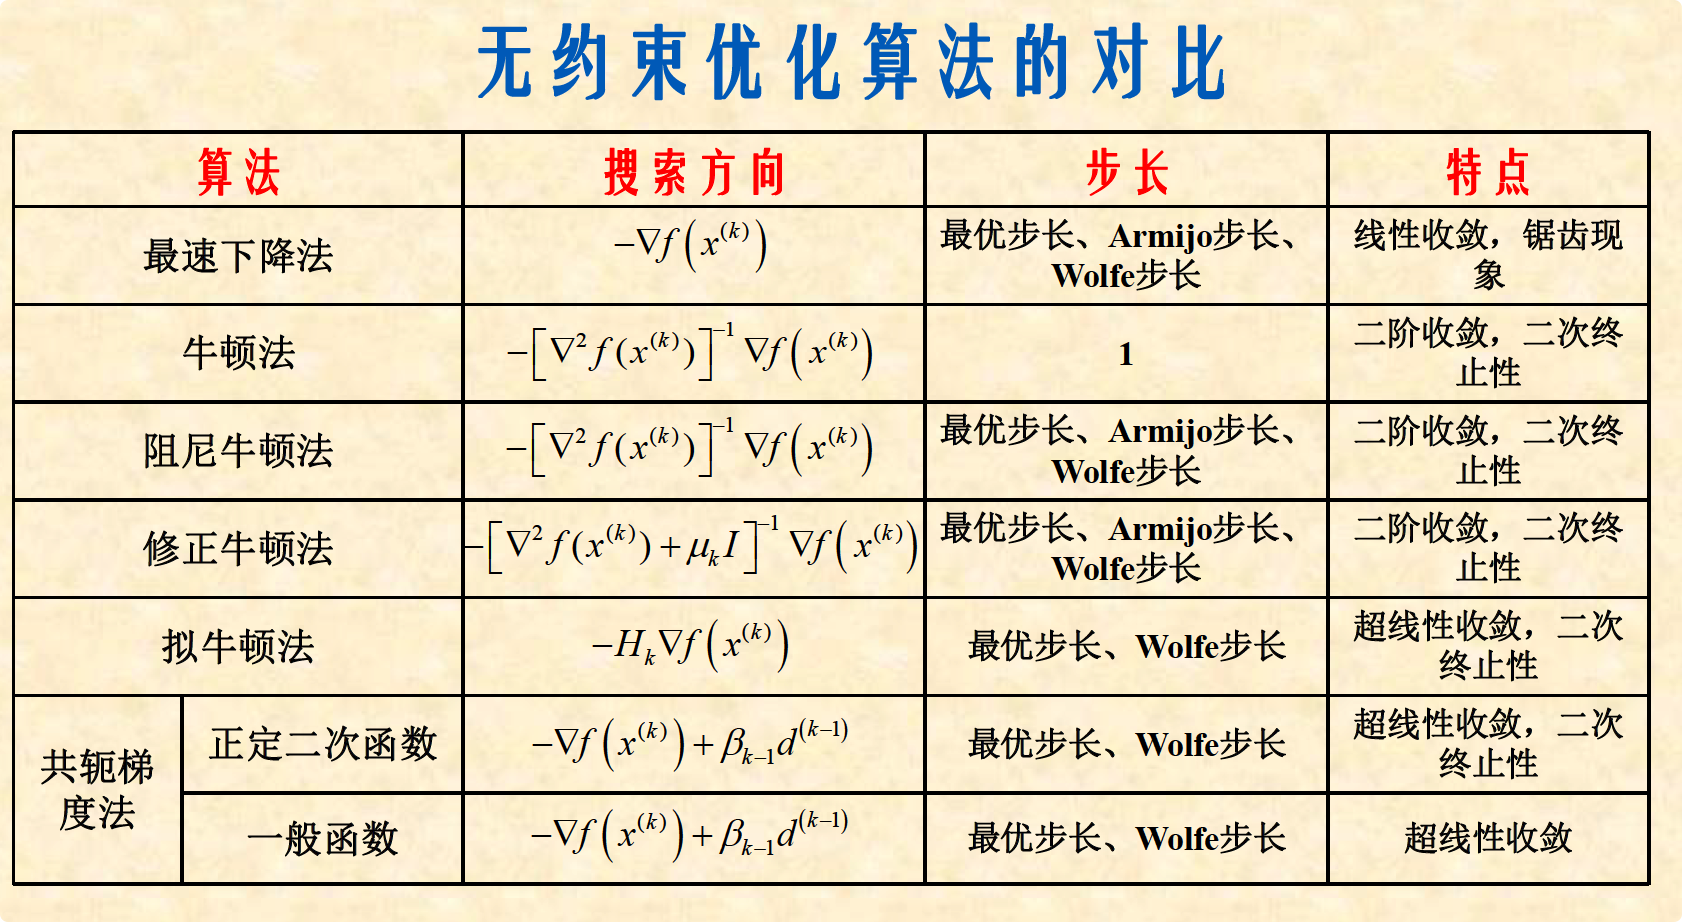
\includegraphics[width=0.8\textwidth]{./figures/img3.png}
    \caption{无约束优化算法的对比 \label{fig3}}
\end{figure}
\newpage
\section{罚函数法}
\textbf{外点罚函数法、内点罚函数法}、乘子罚函数法.

\subsection{外点罚函数法}
\begin{note}
    对于有约束优化问题 \[\begin{cases}
        \min \quad &f(x)\\
        \subject \quad &g_i(x) \ge 0, i = 1, \dots, m\\
        &h_j(x) = 0, j = 1, \dots, l
    \end{cases}\]
    \begin{itemize}
        \item 通过引入罚项转换为无约束优化问题 \begin{align*}
            \min F(x, \sigma) &= f(x) + \sigma p(x)\\
            &= f(x) + \sigma \left(\sum_{i = 1}^m \varphi(g_i(x)) + \sum_{j = 1}^l \psi(h_j(x))\right)
        \end{align*}
        \item 其中 $\sigma$ 是很大的正数,$\varphi(y), \psi(y)$ 是连续函数.
        \item 一般取 $\varphi(g_i(x)) = \left(\max\left\{0, -g_i(x)\right\}\right)^\alpha$,$\psi(h_j(x)) = |h_j(x)|^\beta$,通常 $\alpha = \beta = 2$.
    \end{itemize}
\end{note}

\begin{note}
    外点罚函数法步骤:\begin{enumerate}
        \item 给定初始点 $x^{(0)}$,初始罚因子 $\sigma_1 > 0(\sigma_1 = 1)$,放大系数 $c > 1$,允许误差 $\varepsilon > 0$,置 $k = 1$.
        \item 以 $x^{(k - 1)}$ 为初始点,求解无约束问题 $\min f(x) + \sigma_k p(x)$ 设其极小点为 $x^{(k)}$.
        \item 若 $\sigma_kp(x^{(k)}) < \varepsilon$,则停止计算,得到点 $x^{(k)}$;否则令 $\sigma_{k + 1} = c\sigma_k$,置 $k := k + 1$,返回步骤2.
    \end{enumerate}
\end{note}

\begin{theorem}
    对于由外点法所产生的序列 $\left\{x^{(k)}\right\}$,总有\begin{enumerate}
        \item $F(x^{(k + 1)}, \sigma_{k + 1}) \ge F(x^{(k)}, \sigma_k)$
        \item $p(x^{(k + 1)}) \le p(x^{(k)})$
        \item $f(x^{(k + 1)}) \ge f(x^{(k)})$
    \end{enumerate}
\end{theorem}

\begin{theorem}
    设 $x^*$ 是问题(A)的一个最优解,则对 $\forall k$,有$f(x^*) \ge F(x^{(k)}, \sigma_k) \ge f(x^{(k)})$
\end{theorem}

\begin{note}
    外点罚函数法的重要特点:函数 $F(x, \sigma)$ 是在整个空间 $E^n$ 内进行优化,初始点可任意选择,且外点法也可用于非凸规划的最优化.

    缺点\begin{enumerate}
        \item 惩罚项 $\sigma p(X)$ 的二阶偏导数一般不存在;
        \item 外点法的中间结果不是可行解,不能作为近似解;
        \item 当点 $x^{(k)}$ 接近最优解时,罚因子 $\sigma_k$ 很大.可能使罚函数性质变坏,使搜索产生极大困难.
    \end{enumerate}
\end{note}

\subsection{内点罚函数法}
基本思想:迭代总是从内点出发,并保持在可行域内部进行搜索.

\begin{note}
    障碍函数:\[G(x, r) = f(X) + rB(x)\]
    其中 $r$ 是很小的正数,$B(x)$ 定义在可行域内部,它满足两个条件:\begin{enumerate}
        \item $B(x)$ 是连续函数
        \item 当点 $x$ 趋向可行域边界时,$B(x) \to +\infty$
    \end{enumerate}
    两种最重要的形式:\[B(x) = \sum_{i = 1}^m \frac{1}{g_i(x)} \quad B(x) = -\sum_{i = 1}^m\ln g_i(x)\]
\end{note}

\begin{note}
    算法步骤:\begin{enumerate}
        \item 给定初始点 $x^{(0)} \in \operatorname{int} S$,允许误差 $\varepsilon > 0$,初始参数 $r_1$,缩小系数 $\beta\in (0, 1)$,置 $k=1$.
        \item 以 $x^{(k - 1)}$ 为初始点,求解下列问题\[\begin{cases}
            \min \quad &f(x) + r_kB(x)\\
            \subject \quad &x \in \operatorname{int} S
        \end{cases}\]设其极小点为 $x^{(k)}$.
        \item 若 $r_kB(x^{(k)}) < \varepsilon$,则停止计算,得到点 $x^{(k)}$;否则,令 $r_{k + 1} = \beta r_k$,置 $k := k + 1$,返回2.
    \end{enumerate}
\end{note}

\begin{theorem}
    对于由内点法所产生的序列 $\{x^{(k)}\}$,总有\begin{enumerate}
        \item $G(x^{(k + 1)}, r_{k + 1}) \le G(x^{(k)}, r_k)$
        \item $B(x^{(k + 1)}) \ge B(x^{(k)})$
        \item $f(x^{(k + 1)}) \le f(x^{(k)})$
    \end{enumerate}
\end{theorem}

\begin{theorem}
    设 $\{x^{(l)}\}$ 是由内点法产生的一个序列,则 $\{x^{(k)}\}$ 的任何收敛子序列的极限都是原问题的最优解.
\end{theorem}

\begin{note}
    求初始内点的迭代步骤:\begin{enumerate}
        \item 任取 $x^{(0)} \in E^n, r_0 > 0$(如取 $r_0 = 1$),置 $k := 0$.
        \item 令 $S_k = \left\{i \mid g_i(x^{(k)}) \le 0, 1 \le i \le m\right\}, T_k = \left\{i \mid g_i(x^{k}) > 0, 1 \le i \le m\right\}$
        \item 若 $S_k = \varnothing$,停止计算;否则,转4.
        \item 构造函数 \[\widetilde{P}\left(x, r_{k}\right)=-\sum_{i \in S_{k}} g_{i}(x)+r_{k} \sum_{i \in T_{k}} \frac{1}{g_{i}(x)},\left(r_{k}>0\right)\]
        记 $\widetilde{R}_{k}=\left\{x \mid g_{i}(x)>0 ,i \in T_{k}\right\}$
        \item 以 $x^{(k)}$ 为初始点,在 $\tilde{R_k}$ 域内,求障碍函数 $\tilde{P}(x, r_k)$ 的极小点:\[\begin{cases}
            \min &\tilde{P}(x, r_k)\\
            \subject & x \in \tilde{R_k}
        \end{cases}\] 得 $x^{(k + 1)}$,转6
        \item 令 $ 0 < r_{k + 1} < r_k$ (如取 $r_{k + 1} = \frac{1}{10}r_k$),置$k:=k+1$,转2.
    \end{enumerate}
\end{note}

\begin{note}
    内点罚函数法优点:迭代总在可行域内进行,每一个中间结果都是可行解,可以作为近似解.

    内点罚函数法缺点:选取初始可行点较困难,且只适用于含不等式约束的非线性规划问题,否则没有严格内点.
\end{note}

\subsection{乘子罚函数法}
\subsubsection{等式约束优化的乘子罚函数法}
\begin{note}
    对于等式约束优化问题\[\begin{cases}
        \min &f(x)\\
        \subject &c_i(x) = 0, i \in \varepsilon    
    \end{cases}\]
    $P(x, \lambda, \pi)$ 为乘子罚函数,也称增广 Lagrange 函数.
    \[\min_xP(x, \lambda, \pi) := f(x) - \sum_{i \in \varepsilon}\lambda_ic_i(x) + \pi\sum_{i \in \varepsilon}c_i^2(x)\]
    对于凸规划,任意 $\pi > 0$ 下,原问题的最优解一定是乘子罚函数的最优解.

    并且要使 $c_i(x_k) \to 0$,可以使乘子 $\lambda_i^{(k)}$ 足够靠近最优 Lagrange 乘子 $\lambda_i^*$,而不一定需要罚因子 $\pi_k \to +\infty$.
\end{note}

\begin{note}
    乘子罚函数算法:\begin{enumerate}
        \item 给定 $\pi_0 > 0, \lambda^{(0)} = 0$,初始点 $x_{-1} \in \mathbb{R}^n$,增长因子 $\gamma > 1$ 和允许误差 $\varepsilon > 0$. 令 $k = 0$.
        \item 以 $x_{k - 1}$ 为初始点,用无约束优化方法计算函数 $P(x, \lambda^{(k)}, pi_k)$ 的最小值点 $x_k$.
        \item 若 $\max\{|c_i(x_k)| \mid i \in \varepsilon\} \le \varepsilon$,算法终止. 否则,转下一步.
        \item 若 $\norm{c(x_k)}_\infty \ge \norm{c(x_{k - 1})}_\infty$,令 $\pi_{k + 1} = \gamma \pi_k, \lambda^{(k + 1)} = \lambda_k$,置 $\lambda^{(k + 1)} = \lambda^{(k)}$,转步2. 否则,转步5.
        \item 若 $\pi_k > \pi_{k - 1}$ 或 $\norm{c(x_k)}_\infty \le \frac{1}{4}\norm{c(x_{k - 1})}_\infty$,令 $\pi_{k + 1} = \pi_k$,根据 $\lambda_i^{(k + 1)} = \lambda_i^{(k)} - 2\pi_kc_i(x_k)$ 调整 $\lambda^{(k + 1)}$,置 $k = k + 1$,转步2. 否则,令 $\pi_{k + 1} = \gamma \pi_k$,$\lambda^{(k + 1)} = \lambda^{(k)}$,置 $k = k + 1$,转步2.
    \end{enumerate}
\end{note}



% \nocite{*}
% \printbibliography[heading=bibintoc, title=\ebibname]

% \appendix
% \appendixpage
% \addappheadtotoc

\newpage
\section{最小二乘问题}\newpage

\end{document}